\documentclass[aspectratio=169]{beamer}
\usetheme{Madrid}
\usecolortheme{default}
\usepackage[utf8]{inputenc}
\usepackage[T5]{fontenc}
\usepackage{graphicx}
\usepackage{hyperref}
\usepackage{booktabs}
\usepackage{amsmath}
\usepackage{listings}
\usepackage{xcolor}

\setbeamertemplate{caption}[numbered]
\renewcommand{\figurename}{Hình}
\renewcommand{\thefigure}{14.\arabic{figure}}

\definecolor{codegreen}{rgb}{0,0.6,0}
\definecolor{codegray}{rgb}{0.5,0.5,0.5}
\definecolor{codepurple}{rgb}{0.58,0,0.82}
\definecolor{backcolour}{rgb}{0.95,0.95,0.92}

\lstset{
    backgroundcolor=\color{backcolour},   
    commentstyle=\color{codegreen},
    keywordstyle=\color{magenta},
    numberstyle=\tiny\color{codegray},
    stringstyle=\color{codepurple},
    basicstyle=\ttfamily\scriptsize,
    breakatwhitespace=false,         
    breaklines=true,                 
    captionpos=b,                    
    keepspaces=true,                 
    numbers=left,                    
    numbersep=5pt,                  
    showspaces=false,                
    showstringspaces=false,
    showtabs=false,                  
    tabsize=2
}

\title[Chương 14: Phân loại Văn bản]{Học Sâu (Deep Learning) \\ \vspace{0.5cm} \Large Chương 14: Phân loại Văn bản \\ (Text Classification \& NLP)}
\author{Đại học Đông Á}
\date{\today}

\begin{document}

\begin{frame}
    \titlepage
\end{frame}

\begin{frame}{Nội dung chương}
    \tableofcontents
\end{frame}

\section{1. Giới thiệu Xử lý Ngôn ngữ Tự nhiên (NLP)}

\begin{frame}{Lịch sử và Bản chất của NLP}
    \begin{itemize}
        \item Ngôn ngữ tự nhiên (Tiếng Việt, Tiếng Anh) khác biệt hoàn toàn với ngôn ngữ lập trình (C++, Python). Nó luôn biến động, mập mờ, phức tạp và phá vỡ quy tắc ngữ pháp của chính nó.
        \item \textbf{Natural Language Processing (NLP)} là lĩnh vực giao thoa giữa AI và Ngôn ngữ học nhằm giúp máy tính có thể "đọc", "hiểu" và "giao tiếp" bằng ngôn ngữ con người.
        \item Những năm 1950 - 1990: Thống trị bởi các bộ quy tắc gõ tay (Rule-based / Symbolic AI). Rất cứng nhắc và dễ thất bại.
        \item Cuối 1990 - Nay: Dịch chuyển sang \textbf{Machine Learning \& Statistical NLP} (Mô hình thống kê tự học luật từ dữ liệu).
    \end{itemize}
\end{frame}

\begin{frame}{Các Bài toán Cốt lõi của NLP}
    NLP xử lý một lượng lớn các ứng dụng trong đời sống hiện đại:
    \begin{itemize}
        \item \textbf{Text Classification (Phân loại văn bản):} Email này có phải là Thư rác (Spam) không? Bình luận này mang cảm xúc Tiêu cực hay Tích cực (Sentiment Analysis)?
        \item \textbf{Machine Translation (Dịch máy):} Dịch một câu tiếng Anh sang tiếng Việt sao cho hợp ngữ cảnh nhất (Google Translate).
        \item \textbf{Language Modeling (Mô hình ngôn ngữ):} Cho trước một đoạn văn, hãy dự đoán từ tiếp theo sẽ là gì? (Nền tảng của ChatGPT).
    \end{itemize}
\end{frame}

\section{2. Chuỗi Tiền xử lý Văn bản (Text Pipeline)}

\begin{frame}{Tại sao cần Tiền xử lý Văn bản?}
    \begin{itemize}
        \item Máy tính không hiểu được các ký tự (Char) hay các từ (Word). Mạng Nơ-ron chỉ hoạt động trên các Ma trận và Tensor gồm các \textbf{Con số (Numbers)}.
        \item Do đó, ta phải Vector hóa (Vectorize) văn bản, tức là biến đổi chuỗi văn bản thô thành một chuỗi các con số hoặc một ma trận có cấu trúc.
        \item Quá trình này không thể làm tùy tiện mà phải tuân theo một Chuỗi xử lý (Text Pipeline) nghiêm ngặt gồm 3 bước.
    \end{itemize}
\end{frame}

\begin{frame}{Text Pipeline: 3 Bước Bất di bất dịch}
    \begin{columns}
        \column{0.5\textwidth}
        \begin{enumerate}
            \item \textbf{Standardization (Chuẩn hóa):} Đưa văn bản về một chuẩn chung. Ví dụ: Chuyển toàn bộ thành chữ thường (lower case), xóa bỏ các dấu câu chấm phẩy dư thừa (Punctuation removal).
            \item \textbf{Tokenization (Tách từ):} Chẻ câu văn bản thành các đơn vị rời rạc gọi là "Tokens" (Có thể là Từ, Ký tự, hoặc Cụm từ).
            \item \textbf{Indexing (Đánh chỉ mục):} Chuyển mỗi Token thành một con số duy nhất bằng cách xây dựng Bộ Từ điển (Vocabulary) cho toàn bộ tập dữ liệu.
        \end{enumerate}
        
        \column{0.5\textwidth}
        \begin{figure}
            \centering
            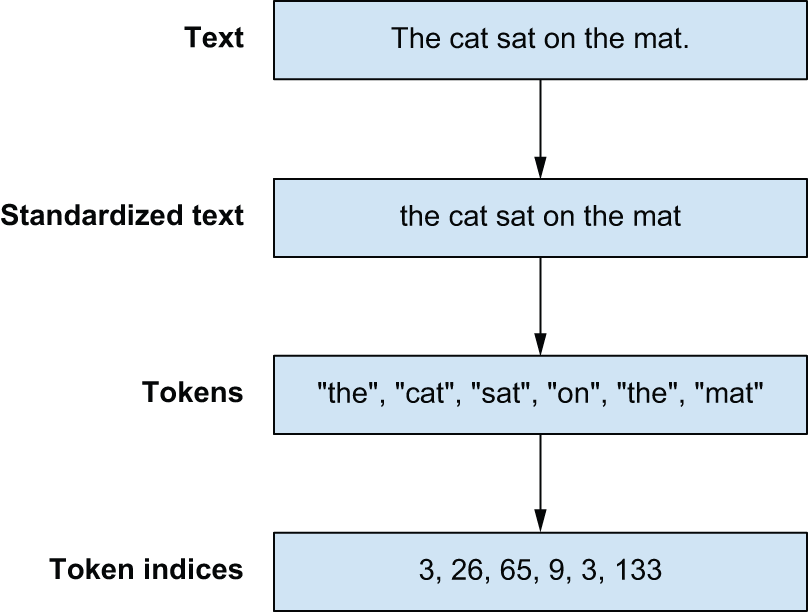
\includegraphics[width=\textwidth,height=0.6\textheight,keepaspectratio]{../../images/ch14/text-pipeline.c09bbad6.png}
            \caption{Tổng quan Quy trình xử lý Văn bản}
        \end{figure}
    \end{columns}
\end{frame}

\begin{frame}[fragile]{Tokenization: Tách ký tự và Tách từ bằng Regex}
Trong Python, \texttt{regex} là công cụ mạnh mẽ nhất để nhận diện mẫu.
\begin{lstlisting}[language=Python]
import regex as re

# 1. Split into characters
def split_chars(text):
    return re.findall(r".", text)

chars = split_chars("The quick brown fox.")
# ["T", "h", "e", " ", "q", "u", "i", "c", "k", " ", ...]

# 2. Split into words and punctuation
def split_words(text):
    # Matches consecutive word characters OR punctuation marks
    return re.findall(r"[\w]+|[.,!?;]", text)

words = split_words("The quick brown fox jumped over the dog.")
# ["The", "quick", "brown", "fox", "jumped", "over", "the", "dog", "."]
\end{lstlisting}
\end{frame}

\begin{frame}[fragile]{Indexing: Xây dựng Từ điển (Vocabulary)}
Kỹ thuật mạnh mẽ nhất là xây dựng ánh xạ từ các mã thông báo cụ thể đến các chỉ mục bằng từ điển (Dictionary / Vocabulary).
\begin{lstlisting}[language=Python]
# Mapping tokens to unique integer indices
vocabulary = {
    "[UNK]": 0, # Unknown token placeholder
    "the": 1,
    "quick": 2,
    "brown": 3,
    "fox": 4,
    "jumped": 5,
    "over": 6,
    "dog": 7,
    ".": 8,
}
words = split_words("The quick brown fox jumped over the lazy dog.")

# Index the tokens. "lazy" becomes 0 because it's not in vocab.
indices = [vocabulary.get(word.lower(), 0) for word in words]
print(indices)
# Output: [1, 2, 3, 4, 5, 6, 1, 0, 7, 8]
\end{lstlisting}
\end{frame}

\begin{frame}{Nhược điểm của Tách Ký tự và Tách Từ}
    \begin{itemize}
        \item \textbf{Cấp độ Ký tự (Char-level):} Từ điển siêu nhỏ (Khoảng 60-100 ký tự ASCII/Unicode) nhưng mỗi câu bị chẻ thành hàng trăm tokens nhỏ lẻ $\rightarrow$ Mất hết ý nghĩa logic, mô hình rất khó học.
        \item \textbf{Cấp độ Từ (Word-level):} Giữ nguyên được ý nghĩa ngữ nghĩa trọn vẹn, chuỗi ngắn gọn. Nhưng từ điển sẽ phình to ra khổng lồ (hàng trăm ngàn từ). Những từ hiếm (Rare words) hoặc sai chính tả sẽ bị gom vào \texttt{[UNK]}.
        \item \textbf{Giải pháp dung hòa:} Mã hóa từ phụ (Sub-word Tokenization).
    \end{itemize}
\end{frame}

\begin{frame}{Mã hóa từ phụ (Sub-word Tokenization) và BPE}
    \begin{itemize}
        \item \textbf{Mục tiêu:} Giữ từ điển nhỏ như Char-level nhưng độ dài chuỗi ngắn như Word-level.
        \item \textbf{Thuật toán BPE (Byte-Pair Encoding):} Bắt đầu với từng ký tự đơn lẻ. Lặp lại việc \textbf{gộp (merge)} 2 ký hiệu xuất hiện cùng nhau nhiều nhất thành một ký hiệu mới.
        \item Ví dụ gộp BPE:
        \begin{itemize}
            \item "l" + "o" $\rightarrow$ "lo"
            \item "lo" + "w" $\rightarrow$ "low"
        \end{itemize}
        \item Đây là thuật toán đứng đằng sau các mô hình khổng lồ như GPT-3, ChatGPT và BERT.
    \end{itemize}
\end{frame}

\begin{frame}[fragile]{Tự động hóa với Keras \texttt{TextVectorization}}
Thay vì tự viết hàm, Keras cung cấp layer \texttt{TextVectorization} siêu việt. Khác với mã thông thường chạy trên CPU, lớp này có thể lồng thẳng vào Model và hoạt động trên GPU/TPU.
\begin{lstlisting}[language=Python]
from keras import layers

# Configure the layer with a maximum vocabulary size
text_vectorization = layers.TextVectorization(
    max_tokens=20000,
    output_mode="int", # Return sequence of token indices
    split="whitespace",
    standardize="lower_and_strip_punctuation"
)

# Build vocabulary directly from a dataset
text_vectorization.adapt(text_dataset)

# Encode a new string
encoded = text_vectorization([["A new text string"]])
\end{lstlisting}
\end{frame}

\section{3. Phương pháp Biểu diễn Túi từ (Bag-of-Words)}

\begin{frame}{Phương pháp Túi từ (Bag-of-Words)}
    \begin{itemize}
        \item Lịch sử NLP bắt đầu với các mô hình \textbf{Set-based (Dựa trên Tập hợp)}.
        \item Thuật toán Bag-of-Words: Chỉ quan tâm từ $X$ xuất hiện \textbf{có mặt hay vắng mặt} trong văn bản, hoàn toàn vứt bỏ trật tự thời gian.
        \item \textbf{Hạn chế chí mạng:} Hai câu "Chó cắn người" và "Người cắn chó" sẽ có chung một vector biểu diễn y hệt nhau, dù ý nghĩa hoàn toàn trái ngược.
        \item Để vớt vát lại thứ tự cục bộ, người ta dùng khái niệm \textbf{N-grams} (Nhóm 2-3 từ liên tiếp nhau). Ví dụ Bi-grams: "Chó cắn", "cắn người".
    \end{itemize}
\end{frame}

\begin{frame}{Thuật toán TF-IDF (Term Frequency-Inverse Document Frequency)}
    \begin{itemize}
        \item Khi dùng Bag-of-Words, các từ như "the", "a", "is", "và", "nhưng" sẽ xuất hiện cực nhiều nhưng mang rất ít giá trị nội dung. Các từ khóa chuyên ngành lại xuất hiện ít nhưng rất giá trị.
        \item \textbf{TF (Term Frequency):} Tần suất từ $t$ xuất hiện trong văn bản hiện tại (Càng nhiều càng tốt).
        \item \textbf{IDF (Inverse Document Frequency):} Nghịch đảo tần suất của từ $t$ trên toàn bộ kho tài liệu (Nói lên độ hiếm có của từ $t$).
        $$ \text{TF-IDF} = TF \times \log\left(\frac{N}{df_t}\right) $$
        \item Nhờ TF-IDF, các từ hiếm sẽ được tăng trọng số, trong khi các từ phổ biến vô nghĩa sẽ bị phạt (đưa về $0$).
    \end{itemize}
\end{frame}

\begin{frame}[fragile]{Áp dụng Bag-of-Words cho tập Dữ liệu IMDb}
Sử dụng \texttt{output\_mode="multi\_hot"} để biến mỗi câu văn bản thành một mảng Zeroes độ dài 20,000. Nếu từ có index $i$ xuất hiện trong câu, giá trị tại vị trí $i$ sẽ là $1$.
\begin{lstlisting}[language=Python]
max_tokens = 20000

# Create multi-hot encoding TextVectorization
text_vectorization = layers.TextVectorization(
    max_tokens=max_tokens,
    split="whitespace",
    output_mode="multi_hot", # Crucial for Bag-of-words
)

# Learn the vocabulary
text_vectorization.adapt(train_ds_no_labels)

# Map the datasets
bag_of_words_train_ds = train_ds.map(
    lambda x, y: (text_vectorization(x), y), num_parallel_calls=8
)
# A batch of 32 outputs has shape (32, 20000)
\end{lstlisting}
\end{frame}

\begin{frame}[fragile]{Xây dựng Linear Classifier cho Bag-of-Words}
Do mỗi đầu vào bây giờ là một \texttt{multi\_hot vector} 20,000 chiều (chứa nhiều số 0 và số 1), ta chỉ cần sử dụng duy nhất một lớp \texttt{Dense} để tính tổng trọng số.
\begin{lstlisting}[language=Python]
import keras

def build_linear_classifier(max_tokens, name):
    inputs = keras.Input(shape=(max_tokens,))
    # A single dense layer for binary classification
    outputs = layers.Dense(1, activation="sigmoid")(inputs)
    model = keras.Model(inputs, outputs, name=name)
    
    model.compile(
        optimizer="adam",
        loss="binary_crossentropy",
        metrics=["accuracy"],
    )
    return model

model = build_linear_classifier(20000, "bag_of_words_classifier")
\end{lstlisting}
\textit{Lưu ý: Mạng này chỉ có 20,001 tham số (Rất nhỏ so với các mạng nơ-ron khác).}
\end{frame}

\begin{frame}{Tiền xử lý hiệu quả với CPU và GPU}
    \begin{itemize}
        \item Quá trình Tiền xử lý văn bản (Regex, Tách từ, Xây dựng từ điển) \textbf{bắt buộc phải chạy trên CPU}. GPU không biết xử lý chuỗi ký tự thô.
        \item Nếu CPU xử lý chậm, GPU đắt tiền sẽ phải "ngồi chờ" (Bottleneck).
        \item \textbf{Giải pháp:} Keras cung cấp \texttt{tf.data.Dataset} cho phép xử lý văn bản đa luồng (Multi-threading) bằng cách chạy song song \texttt{.map()} trên nhiều lõi CPU, cung cấp dữ liệu số liên tục cho GPU học tập.
    \end{itemize}
\end{frame}

\begin{frame}[fragile]{Huấn luyện mô hình Bag-of-Words cơ bản}
Mặc dù là mạng nông, nó huấn luyện nhanh và cực kỳ hiệu quả.
\begin{lstlisting}[language=Python]
# Stop early if validation loss gets worse
early_stopping = keras.callbacks.EarlyStopping(
    monitor="val_loss",
    restore_best_weights=True,
    patience=2,
)

history = model.fit(
    bag_of_words_train_ds,
    validation_data=bag_of_words_val_ds,
    epochs=10,
    callbacks=[early_stopping],
)

# Test Accuracy
test_loss, test_acc = model.evaluate(bag_of_words_test_ds)
print(f"Test Accuracy: {test_acc:.4f}") # Output: 0.8838
\end{lstlisting}
Độ chính xác đạt \textbf{88.38\%} - rất đáng nể với thuật toán ném bỏ toàn bộ thứ tự từ!
\end{frame}

\begin{frame}[fragile]{Tối ưu hóa: Bigram Model (Lưu vết thứ tự cục bộ)}
Ta có thể nâng cấp Bag-of-Words bằng cách sử dụng các cặp 2 từ (Bigrams). Cụm từ "Hoa Kỳ" mang nghĩa khác hoàn toàn chữ "Hoa" và chữ "Kỳ" tách rời.
\begin{lstlisting}[language=Python]
max_tokens = 30000 # Increase vocab size to hold bigrams
text_vectorization = layers.TextVectorization(
    max_tokens=max_tokens,
    split="whitespace",
    output_mode="multi_hot",
    ngrams=2, # Use both Unigrams and Bigrams
)
text_vectorization.adapt(train_ds_no_labels)

# Example vocab learned: ["in a", "most", "him", "dont", "it was", "one of"]
\end{lstlisting}
\textbf{Kết quả:} Sau khi train lại, Accuracy đẩy lên \textbf{90.11\%}.
Nó cực kỳ nhanh nhưng nếu cố tăng n-gram lên quá lớn (ví dụ 4-gram) thì bộ nhớ sẽ cạn kiệt theo cấp số nhân.
\end{frame}

\begin{frame}{Hiệu suất của Bag-of-Words}
    \begin{columns}
        \column{0.5\textwidth}
        \begin{itemize}
            \item Thử nghiệm phân loại cảm xúc tích cực / tiêu cực trên tập dữ liệu IMDB (Đánh giá phim).
            \item Kết hợp Bigrams (N-grams) và mô hình Dense.
            \item \textbf{Kết quả:} Đạt độ chính xác (Accuracy) lên tới hơn 89-90\% trên tập Validation.
            \item Đối với phân loại đơn giản, Bag-of-Words vẫn là một Baseline cực kỳ đáng gờm vì tính nhẹ và cực nhanh của nó.
        \end{itemize}
        
        \column{0.5\textwidth}
        \begin{figure}
            \centering
            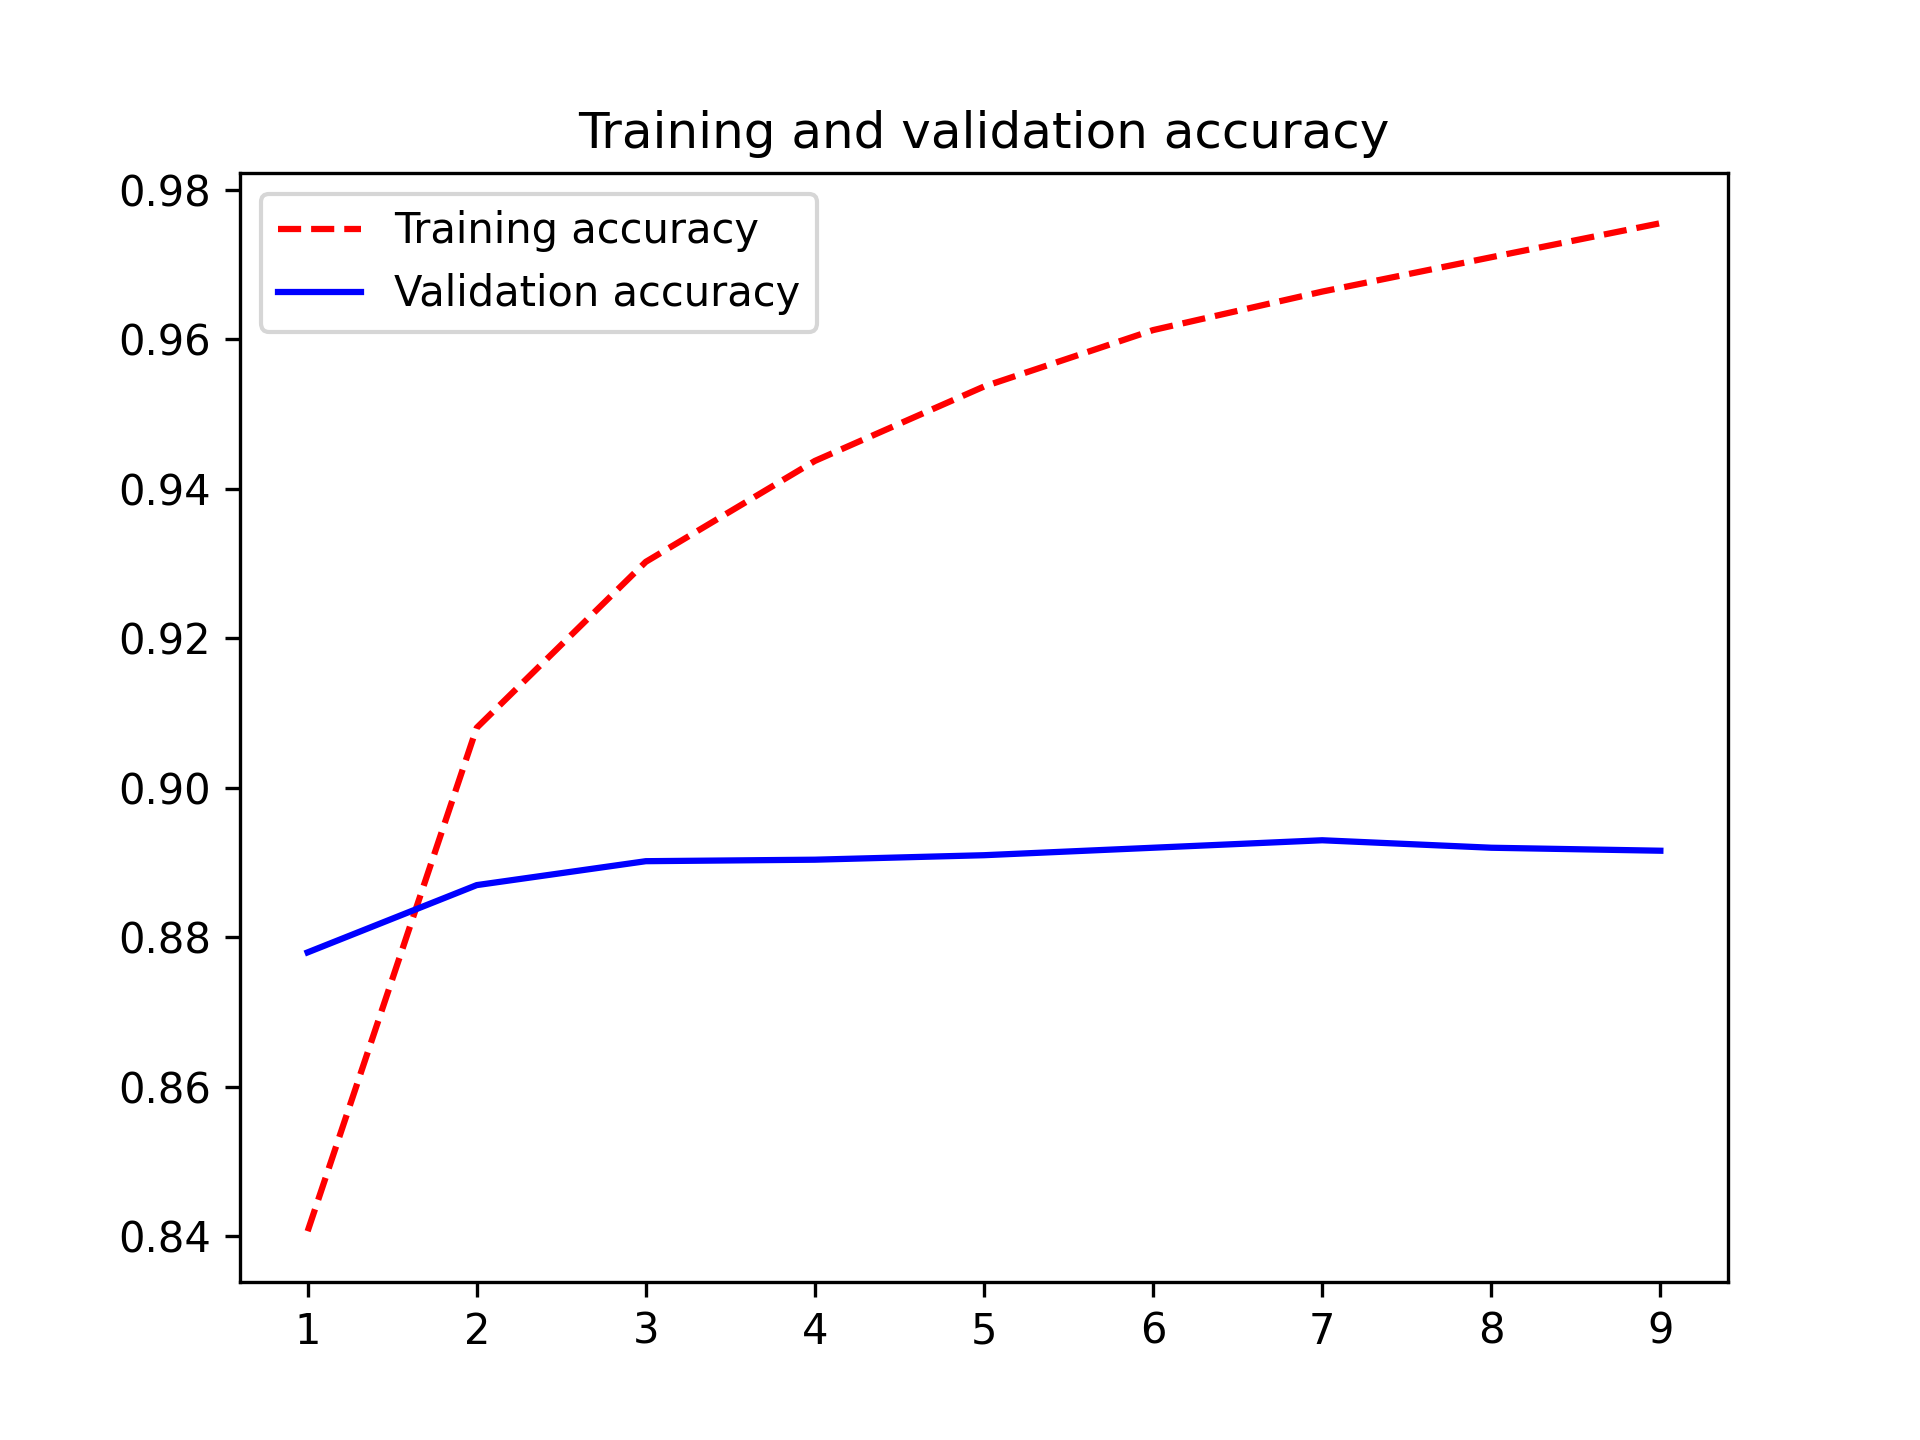
\includegraphics[width=\textwidth,height=0.6\textheight,keepaspectratio]{../../images/ch14/bag-of-words-acc.533d9a5b.png}
            \caption{Độ chính xác của Bag-of-Words}
        \end{figure}
    \end{columns}
\end{frame}

\section{4. Mô hình Trình tự và Word Embeddings - Trái tim của NLP Hiện đại}

\begin{frame}[fragile]{Mô hình Trình tự (Sequence Models)}
Để học tập chuỗi sâu sắc (RNN, LSTM, Transformer), đầu vào bắt buộc phải duy trì theo đúng thời gian tuyến tính. Các câu không bằng nhau cần được Đệm (Padding) hoặc Cắt bỏ (Truncating).
\begin{lstlisting}[language=Python]
max_length = 600 # Force every sequence to be exactly 600 tokens long
max_tokens = 30000

text_vectorization = layers.TextVectorization(
    max_tokens=max_tokens,
    split="whitespace",
    output_mode="int", # Outputs an integer sequence, not a multi_hot set
    output_sequence_length=max_length, # Pad with zeroes if short, cut if long
)
text_vectorization.adapt(train_ds_no_labels)

# Example Output:
# "the slow brown badger" -> ["the", "slow", "brown", "badger", "[PAD]", "[PAD]"]
# -> [1, 255, 331, 840, 0, 0]
\end{lstlisting}
\end{frame}

\begin{frame}{Khuyết điểm của One-hot Encoding}
    \begin{columns}
        \column{0.5\textwidth}
        \begin{itemize}
            \item Trước đây, mỗi từ được biểu diễn bằng One-hot Vector: Một véc-tơ chứa toàn số $0$, chỉ có duy nhất một số $1$.
            \item \textbf{Tính chất rời rạc:} Mọi từ đều độc lập. Khoảng cách toán học (Dot product) giữa từ "Chó" và "Mèo" bằng chính xác khoảng cách giữa "Chó" và "Cái bàn" (Bằng 0).
            \item Mô hình không học được tính chất tương đồng ngữ nghĩa.
        \end{itemize}
        
        \column{0.5\textwidth}
        \begin{figure}
            \centering
            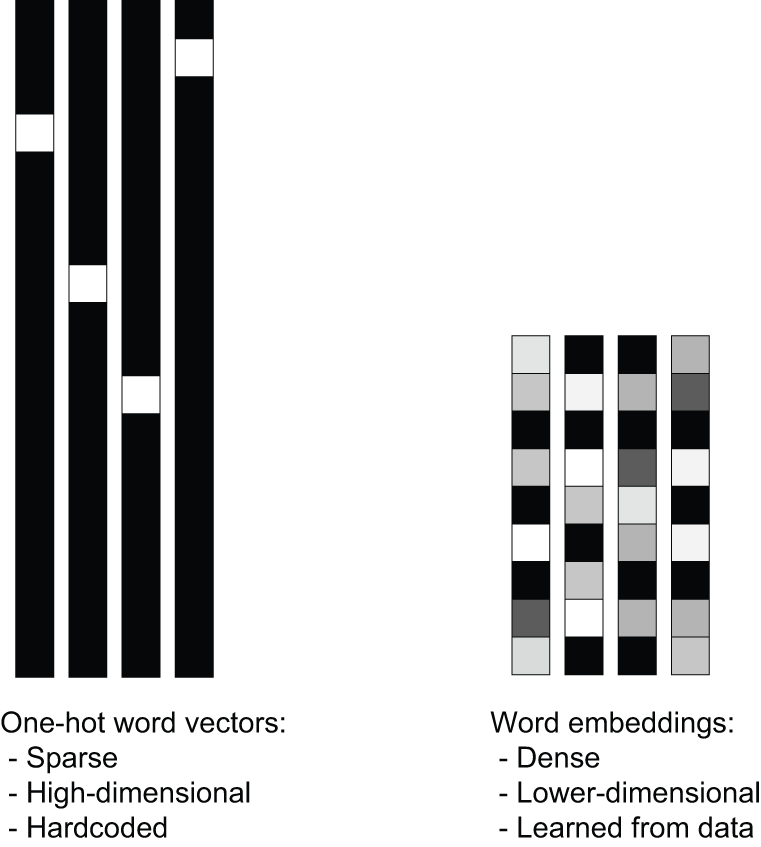
\includegraphics[width=\textwidth,height=0.6\textheight,keepaspectratio]{../../images/ch14/word-representations.b71fcc82.png}
            \caption{Biểu diễn Sparse vs Dense}
        \end{figure}
    \end{columns}
\end{frame}

\begin{frame}{Sự trỗi dậy của Word Embeddings (Nhúng từ)}
    \begin{columns}
        \column{0.5\textwidth}
        \begin{itemize}
            \item \textbf{Word Embeddings} là biểu diễn Dày đặc (Dense), Liên tục (Continuous) mang số thực. Thay vì $10,000$ chiều $0,1$, ta chỉ dùng $256$ chiều số thực.
            \item Những từ có \textbf{Ngữ cảnh giống nhau} sẽ nằm \textbf{Gần nhau} trong không gian hình học đa chiều.
            \item Từ "Dog" và "Wolf" sẽ hội tụ về một góc, khác hoàn toàn với góc của "Car" hay "Bicycle".
        \end{itemize}
        
        \column{0.5\textwidth}
        \begin{figure}
            \centering
            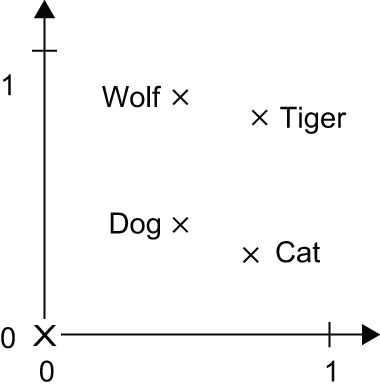
\includegraphics[width=\textwidth,height=0.5\textheight,keepaspectratio]{../../images/ch14/word-embeddings.1bc937b3.png}
            \caption{Không gian Nhúng (Embedding Space)}
        \end{figure}
    \end{columns}
\end{frame}

\begin{frame}{Đại số tuyến tính trong Không gian Ngữ nghĩa}
    \begin{itemize}
        \item Nhờ cấu trúc Dense Vector, mạng Nơ-ron có thể làm \textbf{Toán học trên ngôn ngữ}.
        \item Phép cộng trừ véc-tơ phản ánh chính xác các khái niệm logic của con người:
        \begin{itemize}
            \item Véc-tơ(Vua) - Véc-tơ(Nam) + Véc-tơ(Nữ) = Véc-tơ(Nữ hoàng)
            \item Véc-tơ(Paris) - Véc-tơ(Pháp) + Véc-tơ(Đức) = Véc-tơ(Berlin)
        \end{itemize}
        \item Đây là bước nhảy vọt quan trọng nhất trong lịch sử NLP.
    \end{itemize}
\end{frame}

\begin{frame}{Lớp Embedding (Embedding Layer) trong Keras}
    \begin{columns}
        \column{0.5\textwidth}
        \begin{itemize}
            \item Trong mô hình học sâu, lớp Embedding đóng vai trò như một Cuốn từ điển (Dictionary Lookup).
            \item Đầu vào là một Chỉ mục số nguyên (VD: Từ "Apple" có index là $12$).
            \item Đầu ra là Véc-tơ mang ngữ nghĩa của từ đó tương ứng với Hàng thứ $12$ trong Ma trận trọng số $W$.
            \item Ma trận $W$ này được Cập nhật (Huấn luyện) liên tục qua thuật toán Backpropagation.
        \end{itemize}
        
        \column{0.5\textwidth}
        \begin{figure}
            \centering
            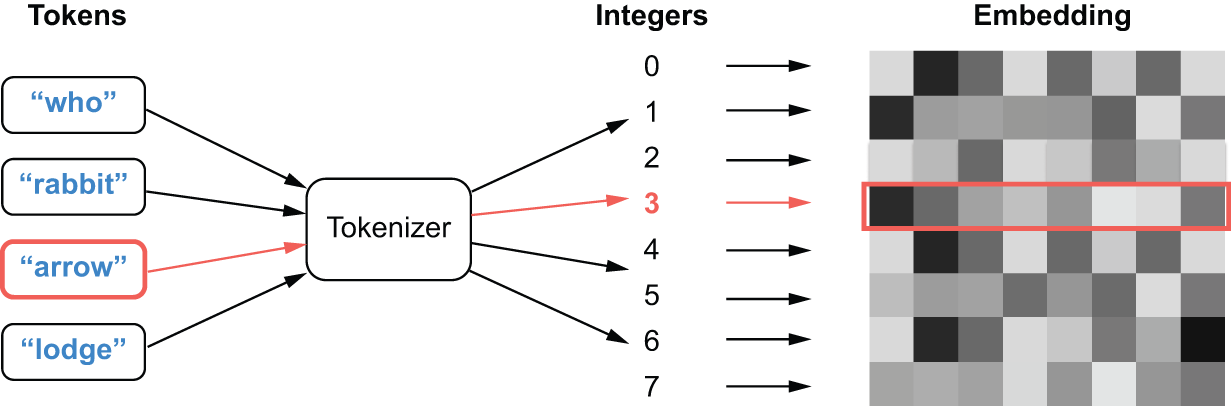
\includegraphics[width=\textwidth,height=0.6\textheight,keepaspectratio]{../../images/ch14/embedding-dictionary.80faa429.png}
            \caption{Cơ chế hoạt động của Lớp Embedding}
        \end{figure}
    \end{columns}
\end{frame}

\begin{frame}[fragile]{Sử dụng \texttt{layers.Embedding} cho mô hình LSTM}
Thêm \texttt{layers.Embedding} trước mạng LSTM để thay đổi dữ liệu từ các Index thành các Không gian Dense liên tục chứa biểu diễn ngữ nghĩa.
\begin{lstlisting}[language=Python]
inputs = keras.Input(shape=(max_length,))

# Embedding Layer translates integer sequences to dense vectors
# Here, each word becomes a 256-dimensional vector
x = layers.Embedding(
    input_dim=max_tokens, 
    output_dim=256,
    mask_zero=True, # Ignore the zeroes generated by padding
)(inputs)

# Now, we can pipe the vectors to a recurrent network
x = layers.Bidirectional(layers.LSTM(32))(x)
x = layers.Dropout(0.5)(x)
outputs = layers.Dense(1, activation="sigmoid")(x)

model = keras.Model(inputs, outputs)
\end{lstlisting}
\end{frame}

\begin{frame}{Vấn đề Dữ liệu Nhãn (Labeled Data) bị hạn chế}
    \begin{itemize}
        \item Lớp \texttt{Embedding} giảm số tham số khổng lồ của một mạng NLP (Từ 15 triệu xuống 2 triệu), mô hình tính toán cực nhanh.
        \item \textbf{Hạn chế:} Trong ví dụ LSTM trước, độ chính xác bị kẹt ở mức $84\%$. Tệ hơn mô hình Bag-of-Words cơ bản.
        \item \textbf{Lý do:} Mạng chứa Embedding + LSTM quá lớn và mạnh. Tập dữ liệu $20,000$ review phim là quá ít để mô hình học được Ngữ nghĩa của thế giới ngôn ngữ rộng lớn. Mô hình bị Overfit nặng (Học thuộc lòng tập train).
        \item \textbf{Giải pháp:} Pre-training (Tiền huấn luyện) không giám sát.
    \end{itemize}
\end{frame}

\begin{frame}{Kiến trúc học Nhúng: Word2Vec và CBOW}
    \begin{columns}
        \column{0.5\textwidth}
        Làm sao có được bộ trọng số Embedding xịn từ đầu? (Pre-trained Word Embeddings).
        \begin{itemize}
            \item Thuật toán **Word2Vec** (Do Tomas Mikolov - Google giới thiệu 2013).
            \item Sử dụng mô hình **CBOW (Continuous Bag-of-Words)**.
            \item Nguyên lý: Ép mô hình \textbf{Dự đoán từ ở giữa} dựa trên các từ ngữ cảnh xung quanh nó (Unsupervised). Trọng số học được sẽ cấu trúc Không gian Vector hợp lý nhất.
        \end{itemize}
        
        \column{0.5\textwidth}
        \begin{figure}
            \centering
            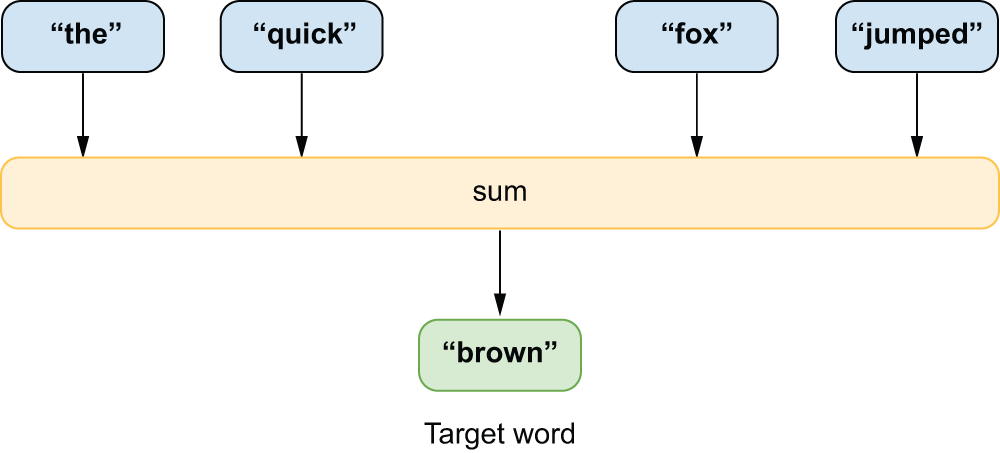
\includegraphics[width=\textwidth,height=0.6\textheight,keepaspectratio]{../../images/ch14/cbow.01aaf529.png}
            \caption{Mô hình dự đoán ngữ cảnh CBOW}
        \end{figure}
    \end{columns}
\end{frame}

\begin{frame}[fragile]{Chuẩn bị dữ liệu Cửa sổ (Context Window) cho CBOW}
Dùng TensorFlow API để cắt nhỏ 1 câu dài thành các túi ngữ cảnh 8 chữ chứa từ mục tiêu bị ẩn.
\begin{lstlisting}[language=Python]
import tensorflow as tf

context_size = 4 # 4 words left, 4 words right
window_size = 9 # Total 9 words in window

# Function to extract label (center word) from context
def split_label(window):
    left = window[:context_size]
    right = window[context_size + 1 :]
    bag = tf.concat((left, right), axis=0) # Shape: 8 context words
    label = window[4] # The word to predict
    return bag, label

# Create sliding windows from text dataset
# [the, quick, brown, FOX, jumped, over, the, lazy] => Label: FOX
dataset = dataset.interleave(window_data)
dataset = dataset.map(split_label)
\end{lstlisting}
\end{frame}

\begin{frame}[fragile]{Xây dựng mô hình CBOW dự đoán nhãn}
Một mạng vô cùng nông kết hợp Embedding và Pool Average. Sau đó huấn luyện trên hàng triệu Text tự do. Vector Embedding thu được sẽ mang thông tin cấu trúc Ngôn ngữ tuyệt vời để cấy vào LSTM.
\begin{lstlisting}[language=Python]
hidden_dim = 64
inputs = keras.Input(shape=(2 * context_size,)) # 8 inputs

# The core embedding layer we want to train
cbow_embedding = layers.Embedding(max_tokens, hidden_dim)
x = cbow_embedding(inputs) # Shape: (8, 64)

# Average all 8 vectors into a single 64-dim vector
x = layers.GlobalAveragePooling1D()(x)

# Predict the word out of the entire dictionary 
outputs = layers.Dense(max_tokens, activation="sigmoid")(x)

cbow_model = keras.Model(inputs, outputs)
cbow_model.compile(loss="sparse_categorical_crossentropy", optimizer="adam")
\end{lstlisting}
\end{frame}

\begin{frame}[fragile]{Sử dụng Pre-trained Embeddings}
Thay vì train Embedding từ đầu trên 20k review, ta có thể tải Embedding đã được train trên toàn bộ Wikipedia (GloVe, Word2Vec) và cắm vào layer.
\begin{lstlisting}[language=Python]
import numpy as np

# Load pretrained weights into the Embedding layer
embedding_layer = layers.Embedding(
    max_tokens,
    256,
    embeddings_initializer=keras.initializers.Constant(pretrained_matrix),
    trainable=False, # Freeze the layer!
)

# Build LSTM model
inputs = keras.Input(shape=(max_length,))
x = embedding_layer(inputs)
x = layers.Bidirectional(layers.LSTM(32))(x)
outputs = layers.Dense(1, activation="sigmoid")(x)
\end{lstlisting}
\end{frame}

\begin{frame}{Sự lựa chọn giữa Set-based và Sequence-based}
    \begin{itemize}
        \item \textbf{Bag-of-Words (Sets):} Sử dụng khi cần train cực nhanh, hoặc chỉ quan tâm đến các \textbf{từ khóa} trong câu hơn là ngữ cảnh sâu xa (Phân tích cảm xúc đơn giản, Lọc Spam).
        \item \textbf{Sequence Models (RNN, LSTM, Transformer):} Sử dụng khi \textbf{trật tự từ} quyết định ý nghĩa câu (Dịch máy, Tạo văn bản, Trả lời câu hỏi). Yêu cầu lượng lớn dữ liệu để không bị Overfitting.
        \item Nếu tập dữ liệu $\leq$ 100,000 mẫu, dùng Set-based (Bigrams) kết hợp mạng Dense nhỏ là lựa chọn khôn ngoan nhất.
    \end{itemize}
\end{frame}


\section{Tổng kết}

\begin{frame}{Tổng kết Chương 14}
    \begin{itemize}
        \item Máy tính không hiểu văn bản thô. Cần có **Text Pipeline** (Chuẩn hóa $\rightarrow$ Tách từ $\rightarrow$ Đánh chỉ mục).
        \item **Bag-of-Words / N-grams + TF-IDF:** Đơn giản, cực nhẹ, hiệu quả cao trong phân loại văn bản nhanh, nhưng không nhớ được cấu trúc thời gian của câu.
        \item **Word Embeddings (Nhúng từ):** Là bước đệm vĩ đại của NLP. Chuyển từ sang Không gian Vector Ngữ nghĩa liên tục đa chiều (Toán học hóa ngôn ngữ).
        \item Thuật toán như Word2Vec (CBOW, Skip-gram) giúp khai thác triệt để tài nguyên text khổng lồ trên Internet mà không cần nhãn (Unsupervised learning).
    \end{itemize}
\end{frame}

\end{document}
